
\documentclass[11pt]{amsart}

%\usepackage{color,graphicx}
%\usepackage{mathrsfs,amsbsy}
\usepackage{amssymb}
\usepackage{amsmath}
\usepackage{amsfonts}
\usepackage{bm}
\usepackage{graphicx}
\usepackage{amsthm}
\usepackage{enumerate}
\usepackage[mathscr]{eucal}
\usepackage{float}
\usepackage{mathrsfs}
\usepackage{multicol}
\usepackage[all,pdf]{xy}
\usepackage[a4paper,left=3cm,right=3cm]{geometry}
%\usepackage[notcite,notref]{showkeys}

% showkeys  make label explicit on the paper

\makeatletter
\@namedef{subjclassname@2010}{%
  \textup{2010} Mathematics Subject Classification}
\makeatother

\numberwithin{equation}{section}

\theoremstyle{plain}
\newtheorem{theorem}{Theorem}[section]
\newtheorem{lemma}[theorem]{Lemma}
\newtheorem{proposition}[theorem]{Proposition}
\newtheorem{corollary}[theorem]{Corollary}
\newtheorem{claim}[theorem]{Claim}
\newtheorem{defn}[theorem]{Definition}
\newtheorem{ques}[theorem]{Question}
\newtheorem*{fact}{Facts}
\newtheorem{eg}[theorem]{Example}

\theoremstyle{plain}
\newtheorem{thmsub}{Theorem}[subsection]
\newtheorem{lemmasub}[thmsub]{Lemma}
\newtheorem{corollarysub}[thmsub]{Corollary}
\newtheorem{propositionsub}[thmsub]{Proposition}
\newtheorem{defnsub}[thmsub]{Definition}

\numberwithin{equation}{section}


\theoremstyle{remark}
\newtheorem{remark}[theorem]{Remark}
\newtheorem{remarks}{Remarks}

\newcommand*\widebar[1]{%
	\hbox{%
		\vbox{%
			\hrule height 0.5pt % The actual bar
			\kern0.6ex%         % Distance between bar and symbol
			\hbox{%
				\kern 0em%      % Shortening on the left side
				\ensuremath{#1}%
				\kern 0em%      % Shortening on the right side
			}%
		}%
	}%
}
\makeatletter
\newcommand*{\Relbarfill@}{\arrowfill@\Relbar\Relbar\Relbar}
\newcommand*{\xeq}[2][]{\ext@arrow 0055\Relbarfill@{#1}{#2}}
\makeatother%longarrows
\renewcommand\thefootnote{\fnsymbol{footnote}}
%dont use number as footnote symbol, use this command to change

\DeclareMathOperator{\supp}{supp}
\DeclareMathOperator{\dist}{dist}
\DeclareMathOperator{\vol}{vol}
\DeclareMathOperator{\diag}{diag}
\DeclareMathOperator{\tr}{tr}

\begin{document}
\date{}

\title
{Schur-Horn theorem}


\author{Xiaoxiang Zhou}
\address{School of Mathematical Sciences\\
University of Science and Technology of China\\
Hefei, 230026\\ P.R. China\\} 
\email{email:xx352229@mail.ustc.edu.cn}





\begin{abstract}
In this article, I will use the Atiyah-Guillemin-Sternberg Convexity theorem to prove the Schur-Horn theorem, which is a beautiful theorem in linear algebra, with deep symplectic geometry theory behind it. To introduce the AGM theorem, we first grasp the tools: the Lie bracket and the Exponential map; then we will focus on the vector field induced by the group action $\mathbb{T}^n  \text{ \rotatebox[origin=c]{270}{$\circlearrowleft$} } \mathcal{H}_\lambda$, and use the symplectic structure on $\mathcal{H}_\lambda$ to convert the vector field to an exact 1-form, and then natually introduce the moment map on $\mathcal{H}_\lambda$. After that, we will state the AGM theorem and prove the Schur-Horn theorem.
\end{abstract}

\maketitle
%%%%%%%%%%%%%%%%%%%%%%%%%%%%%%%%%%%%%%%%%%%%%%%%%%%%%%%%%%%%%%%%%%%%%%%%%%%%%%%%%%%%%%%%%%%%%
\vspace{-1cm}%
\section{Introduction}
Given a Hermitian matrix $A=(a_{ij})\in \mathbb{C}^n$
with eigenvalues
$$\bm{\lambda} = (\lambda_1,\lambda_2,\ldots,\lambda_n)^T \in \mathbb{R}^n$$
We want to see:

%\fbox{
%\parbox{\textwidth}{
%}
%}

Question:What do the diagonal elements
$$(a_{11},a_{22},\ldots,a_{nn})$$  
look like?

\begin{fact}(Obvious)
	\begin{itemize}
		\item $A^H=A \Rightarrow a_{11},a_{22},\ldots,a_{nn} \in \mathbb{R}$
		\item $A$ is \textbf{unitary similar} to $\diag(\lambda_1,\ldots,\lambda_n)$ \\
		$\Rightarrow \sum_{i=1}^n a_{ii} = \tr A = tr (\diag(\lambda_1,\ldots,\lambda_n))= \sum_{i=1}^n \lambda_i$
		\item $\forall\; \tau \in S_n, \diag (\lambda_1,\ldots,\lambda_n)$ is unitary similar to
		$\diag (\lambda_{\tau(1)},\ldots,\lambda_{\tau(n)})$ \\
		$\Rightarrow$ WLOG, we can rearrange $(\lambda_1,\ldots,\lambda_n)$ s.t.
		$$\lambda_1 \geqslant \lambda_2\geqslant\ldots\geqslant\lambda_n$$
		NOTICE:After that we will assume $\lambda_1 \geqslant \lambda_2\geqslant\ldots\geqslant\lambda_n$.
	\end{itemize}
\end{fact}
\begin{fact}(Not Obvious)
	\begin{itemize}
		\item $\forall\; i \in \{1,\ldots, n\}, \lambda_n \leqslant a_{ii} \leqslant \lambda_1$
		\item $\forall\; k \in \{1,\ldots, n\}, \sum_{i=1}^k a_{ii} \leqslant \sum_{i=1}^k \lambda_i$ 
		\footnote{Issai Schur (Russian,1875-1941) proved the above-mentioned
			inequalities in 1923.}
	\end{itemize}
\end{fact}
Denote
\begin{align*}
	&\bm{\lambda} =(\lambda_1,\lambda_2,\ldots,\lambda_n)^T \in \mathbb{R}^n \\
	&\Lambda =\diag (\lambda_1,\lambda_2,\ldots,\lambda_n)^T \in \mathbb{R}^{n \times n} \\
	&\mathcal{H} (n)=\{A \in \mathbb{C}^{n \times n} \mid A^H=A\} \\
	&\mathcal{H}_\lambda=\{A \in \mathcal{H} (n) \mid A \text{ is unitary similar to } \Lambda\} \\
	\end{align*}
\begin{equation*}
	\begin{aligned}	
		\pi \colon & \qquad \mathcal{H} (n) &\longrightarrow &\hspace{1.3cm}  \mathbb{R}^n \\
		&A=(a_{ij})_{i,j=1}^n &\mapsto \hspace{0.3cm}&(a_{11},a_{22},\ldots,a_{nn})^T
	\end{aligned}
\end{equation*}

\begin{theorem}(Schur-Horn)
	$\pi (\mathcal{H}_\lambda)$ is a \textbf{convex polyhedron} in $\mathbb{R}^n$ whose vertices are
	$$(\lambda_{\tau(1)},\ldots,\lambda_{\tau(n)})^T \in \mathbb{R}^n$$
	where $\tau \in S_n$.\footnote{Alfred Horn (Amerian, UCLA) proved it in 1954.}
\end{theorem}
With these facts in mind, we will first discuss some examples.
\begin{eg}(trivial)
	when $\bm{\lambda} =(\lambda_0,\lambda_0,\ldots,\lambda_0)^T$, we have
\begin{align*}
	\Lambda \,\,&= \lambda_0 I \\
	\mathcal{H}_\lambda &= \{A \in \mathbb{C}^{n \times n} \mid 
	\exists\; U \in U(n), A=U(\lambda_0 I)U^H = \lambda_0 I\} \\
	 &=\{\lambda_0 I\} \hspace{4.5cm} \text{has only one element!}
\end{align*}	
\end{eg}
 We leave 2-dimension example at last because it’s computable.

\begin{eg}(3-dimension condition)

	when $\bm{\lambda} =(\lambda_1,\lambda_2,\lambda_3)^T$, it's almost impossible to calculate, so we only draw out the final result:
	  	\begin{figure}[H]
	 	\begin{minipage}[t]{.49\textwidth}
	 		\centering
	 		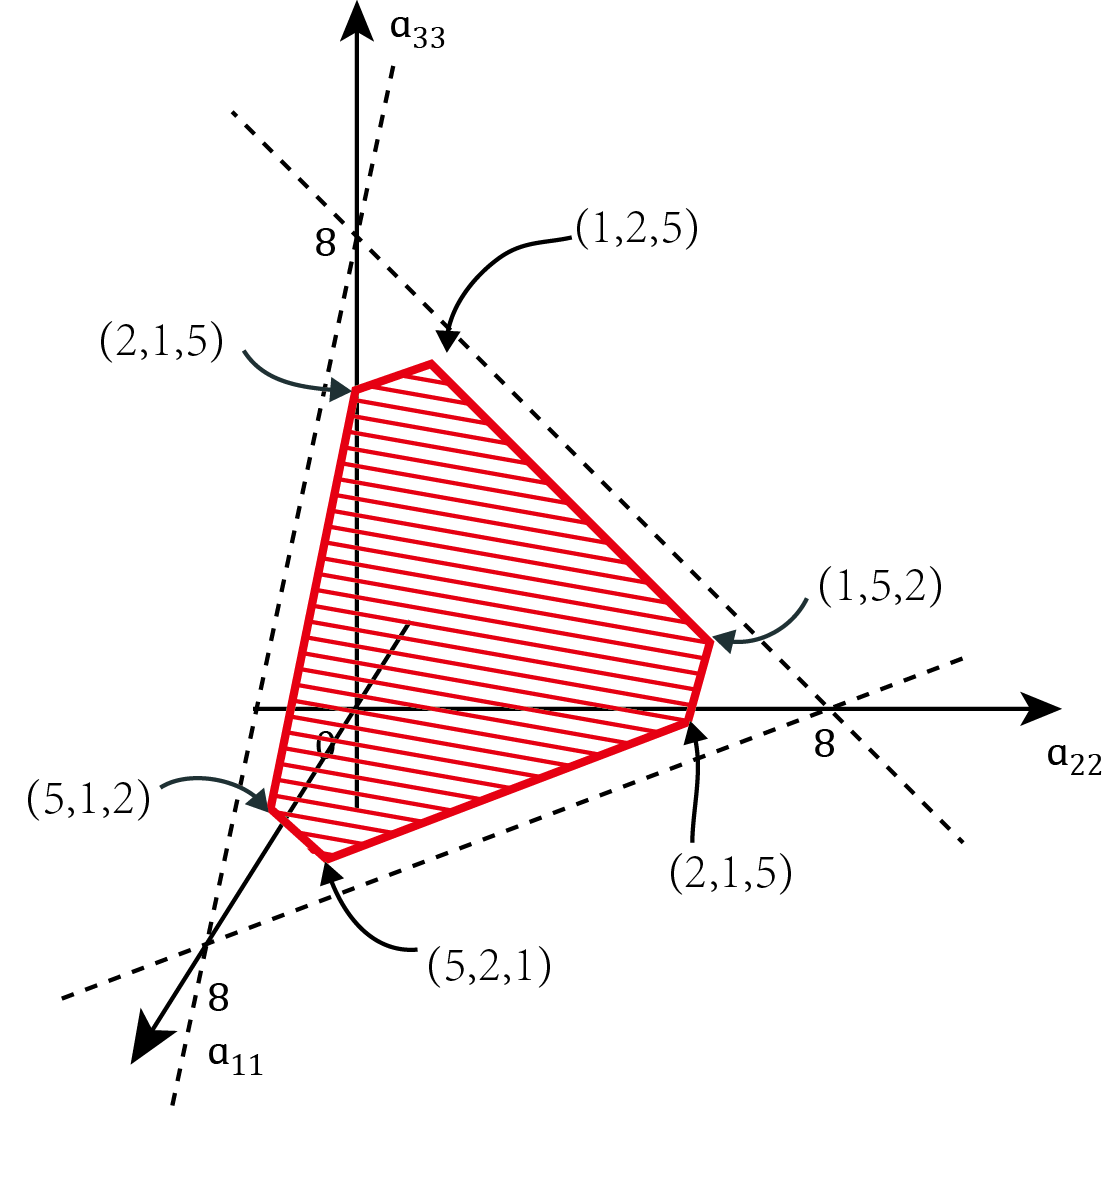
\includegraphics[width=.95\textwidth]{figures/figure4.png}\\
	 		$(\lambda_1,\lambda_2,\lambda_3)^T=(5,2,1)^T$
	 	\end{minipage}
	 	\begin{minipage}[t]{.49\textwidth}
	 		\centering
	 		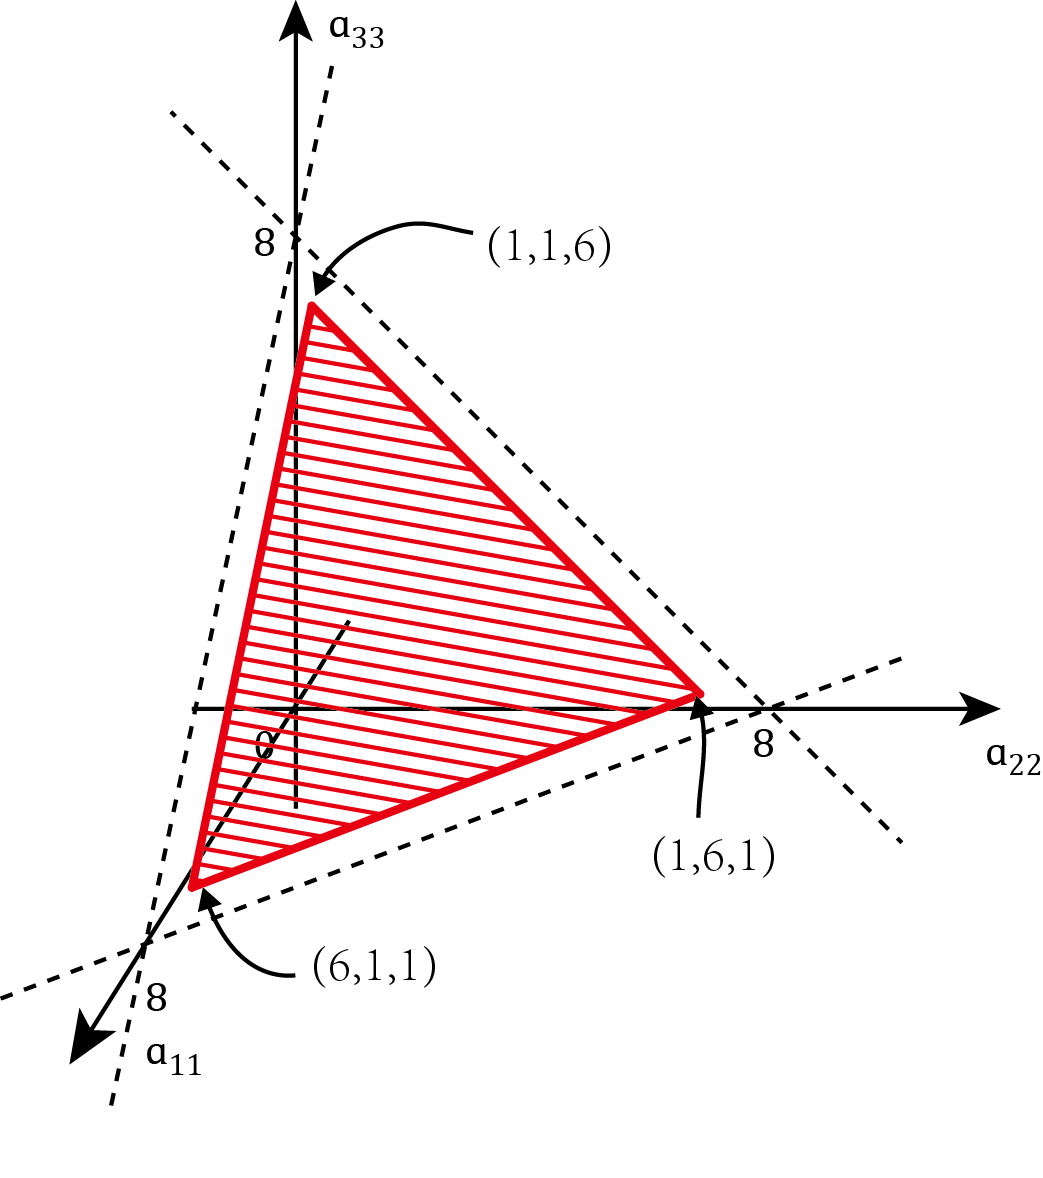
\includegraphics[width=.95\textwidth]{figures/figure3.png}\\
	 		$(\lambda_1,\lambda_2,\lambda_3)^T=(6,1,1)^T$\\"degenerate"
	 	\end{minipage}
	 \end{figure}	
\end{eg}
\begin{eg}(2-dimension condition)
	we have
	$$A= \begin{pmatrix}
	a_{11} & a_{12} \\
	a_{21} & a_{22}
	\end{pmatrix}
	 \in \mathcal{H}_\lambda \Leftrightarrow \exists \;
	 U=\begin{pmatrix}
	 u_{11} & u_{12} \\
	 u_{21} & u_{22}
	 \end{pmatrix}
	 \in U(2),$$
\begin{equation*}
 	\begin{aligned}
 	A&= U\Lambda U^H \\ 	
 	&=\begin{pmatrix}
 	u_{11} & u_{12} \\
 	u_{21} & u_{22}
 	\end{pmatrix}
 	\begin{pmatrix}
 	\lambda_1 &  \\
 	& \lambda_2
 	\end{pmatrix}
 	\begin{pmatrix}
 	\widebar{u_{11}} & \widebar{u_{21}} \\
 	\widebar{u_{12}} & \widebar{u_{22}}
 	\end{pmatrix} \\
 	&=\begin{pmatrix}
 	\lambda_1|u_{11}|^2+\lambda_2 |u_{12}|^2 & \lambda_1  u_{11} \widebar{u_{21}}+\lambda_2 u_{12} \widebar{u_{21}} \\
 	\lambda_1 u_{21} \widebar{u_{11}}+\lambda_2 u_{22} \widebar{u_{12}} & \lambda_1|u_{21}|^2+\lambda_2 |u_{22}|^2
 	\end{pmatrix} \\
 	&=\lambda_2 I + (\lambda_1 - \lambda_2)
 	\begin{pmatrix}
 	|u_{11}|^2 & u_{11} \widebar{u_{21}} \\
 	\lambda_1 u_{21} \widebar{u_{11}} & \lambda_1|u_{21}|^2
 	\end{pmatrix}
 	\end{aligned}
\end{equation*}
	  	\begin{figure}[th]
	\begin{minipage}[t]{.49\textwidth}
		\centering
		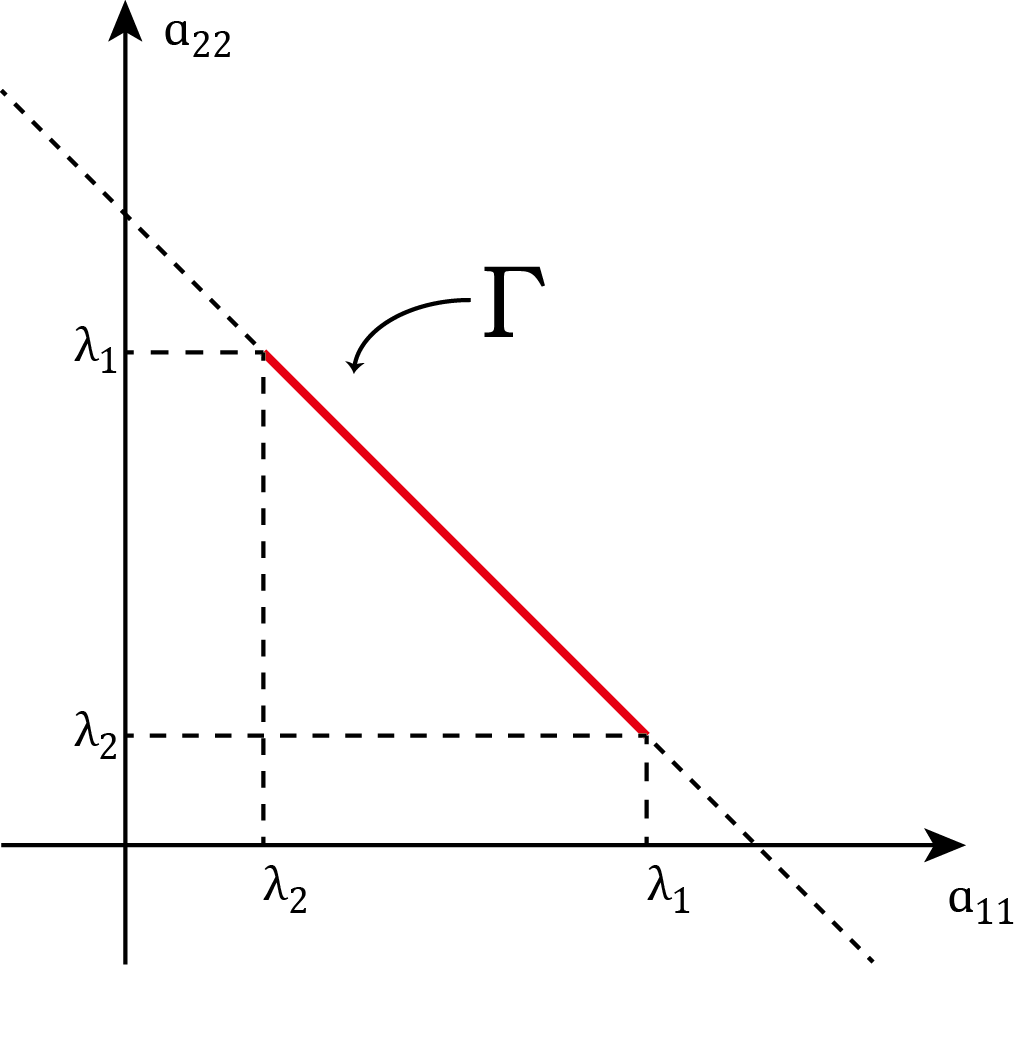
\includegraphics[width=.95\textwidth]{figures/figure1.png}\\
		\caption{}
		\label{fig3}
	\end{minipage}
	\begin{minipage}[t]{.49\textwidth}
		\centering
		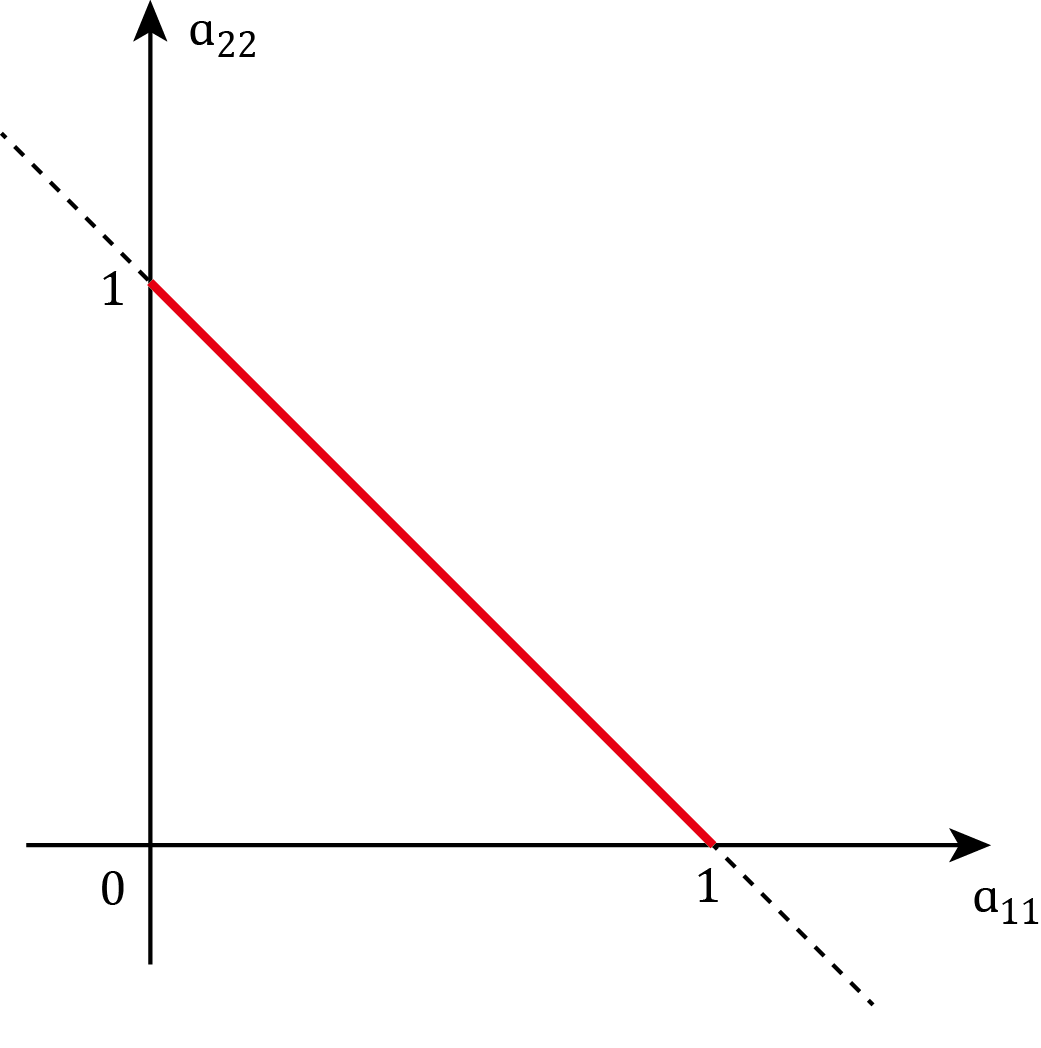
\includegraphics[width=.95\textwidth]{figures/figure2.png}\\
		\caption{}
		\label{fig4}
	\end{minipage}
\end{figure}	
Denote the line segment drawed in the figure \ref{fig3} as $\Gamma$, then
\begin{itemize}
	\item $\pi (\mathcal{H}_\lambda) \subseteq \Gamma$ because 
	$\lambda_1|u_{11}|^2+\lambda_2 |u_{12}|^2$ is the convex combination of $\lambda_1, \lambda_2$.
	\item $\Gamma \subseteq \pi (\mathcal{H}_\lambda)$ because we can take
	$$\begin{pmatrix}
	 u_{11} &  u_{21} \\
	 u_{12} &  u_{22}
	\end{pmatrix}=
	\begin{pmatrix}
	\cos \theta & -\sin \theta \\
	\sin \theta & \cos \theta
	\end{pmatrix}$$.
\end{itemize}

	 Actually one can compute more:
	 
	WLOG(or take the coordinate trasformation), we only consider the condition when 
\begin{itemize}
	\item $\bm{\lambda} =(\lambda_1,\lambda_2)^T=(1,0)^T$ 
	\item 
	$A=\begin{pmatrix}
	|u_{11}|^2 & u_{11} \widebar{u_{21}} \\
	\lambda_1 u_{21} \widebar{u_{11}} & \lambda_1|u_{21}|^2
	\end{pmatrix}$.
\end{itemize}	
Now we can calculate out
$$\mathcal{H}_\lambda = \left\{ 
	\begin{pmatrix}
	a & e^{i\varphi} \sqrt{a(1-a)} \\
	e^{-i\varphi} \sqrt{a(1-a)} & 1-a
	\end{pmatrix} \bigg|a \in [0,1], 0 \leqslant \varphi <2\pi
	\right\} $$
Now we know explicitly
$$\pi (\mathcal{H}_\lambda)=\{(a,1-a) \mid 0\leqslant a \leqslant 1\}$$
Moreover, $\pi (\mathcal{H}_\lambda)$ is a manifold diffeomorphic to $S^2$:
\begin{equation*}
\begin{aligned}	
\Phi \colon &\hspace{2.7cm} \mathcal{H}_\lambda &\longrightarrow &\hspace{.4cm}  S^2 \\
&\begin{pmatrix}
a & e^{i\varphi} \sqrt{a(1-a)} \\
e^{-i\varphi} \sqrt{a(1-a)} & 1-a
\end{pmatrix}\hspace{-0.5cm} &\mapsto &\;(\varphi , a)
\end{aligned}
\end{equation*}

\end{eg}

\begin{remark}
What is a manifold? Manifold is a VERY GOOD geometric object which always look like $R^n$.
\end{remark}
We will find out more information through this isomorphism.	
		  	\begin{figure}[ht]
	\begin{minipage}[t]{.49\textwidth}
		\centering
		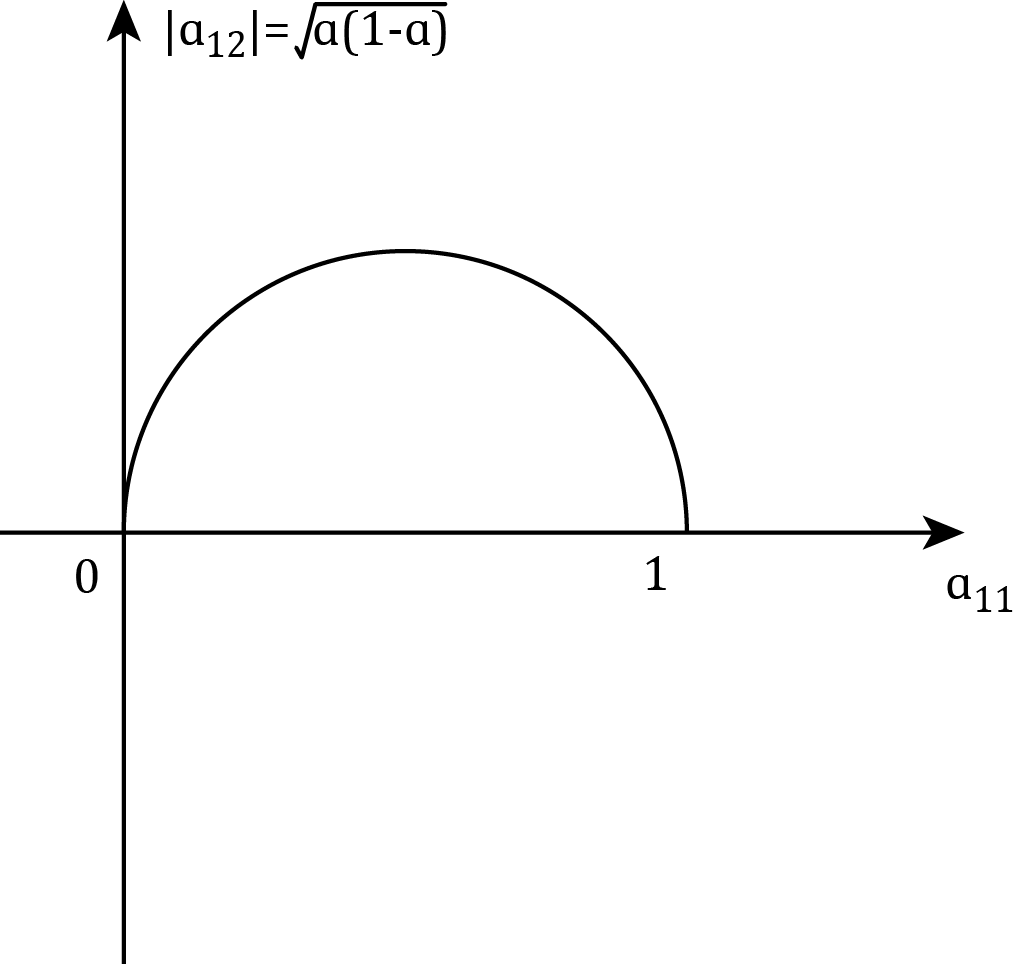
\includegraphics[width=.91\textwidth]{figures/figure5.png}\\
		\caption{}
		\label{fig5}
	\end{minipage}
	\begin{minipage}[t]{.49\textwidth}
		\centering
		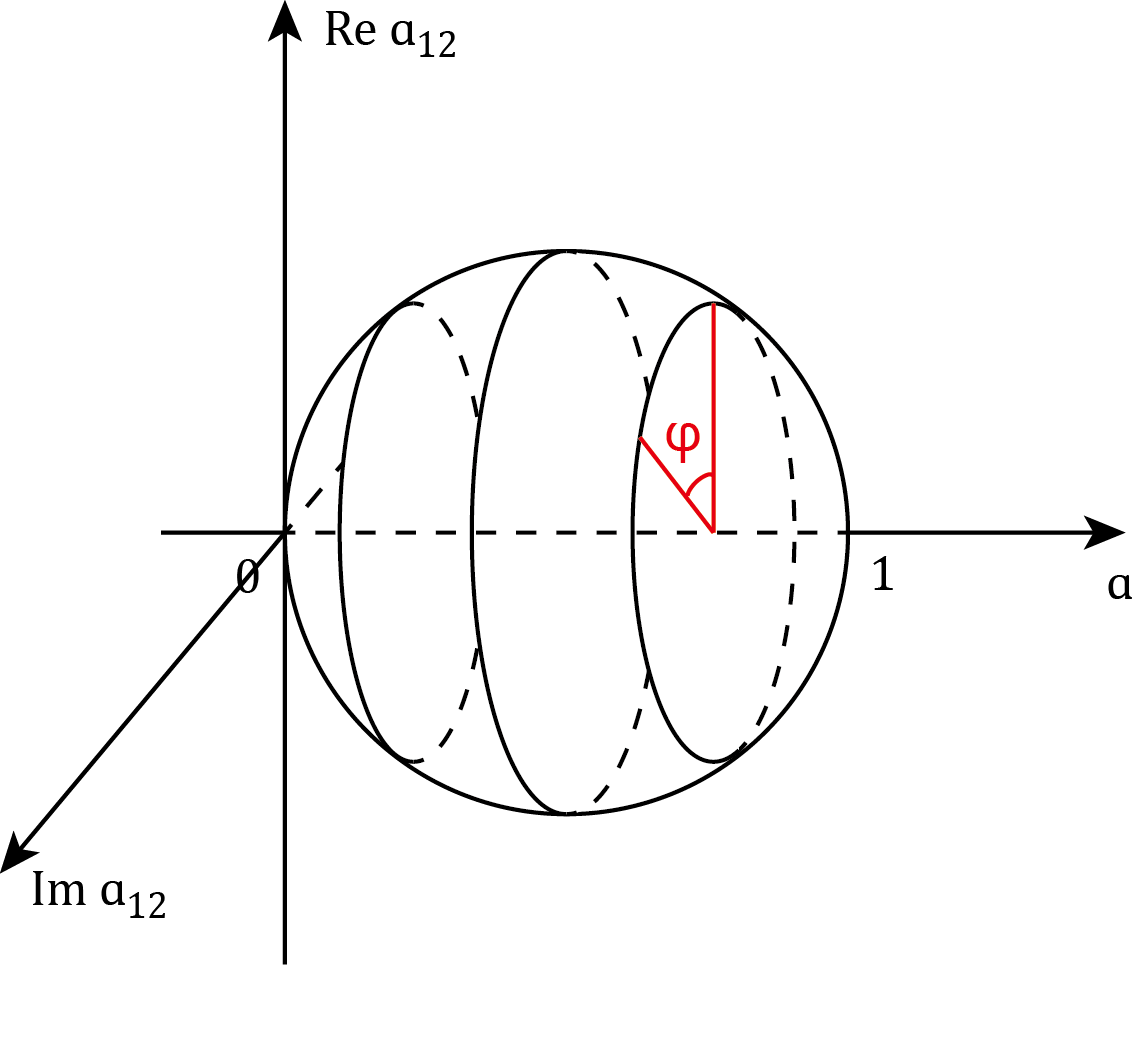
\includegraphics[width=.95\textwidth]{figures/figure6.png}\\
		\caption{}
		\label{fig6}
	\end{minipage}
\end{figure}

\section{Simple Tools}
Let us deriate from the phenomenon for a while to obtain the most basic tools:the \textbf{Lie bracket} and the \textbf{Exponential map}.
\subsection*{Lie bracket}
\begin{defn}
	the Lie bracket of $M_n(\mathbb{C})$ is
	\begin{equation*}
	\begin{aligned}{}
	[\phantom{A},\phantom{B}] \colon  M_n(&\mathbb{C}) \times  M_n(\mathbb{C})\; \longrightarrow \hspace{1.3cm}  \mathbb{C} \\
	&\;(A,B)\hspace{0.6cm} \mapsto \hspace{0.3cm}[A,B]:=AB-BA
	\end{aligned}
	\end{equation*}
\end{defn}
\begin{proposition}
	For any $c_1,c_2 \in \mathbb{C},A,A_1,A_2,B,C \in M_n(\mathbb{C})$, we have the following properties:
	\begin{itemize}
		\item (Skew-Symmetric) $[A,B]=-[B,A]$;
		\item (Linear) $[c_1A_1+c_2A_2,B]=c_1[A_1,B]+c_2[A_2,B]$;
		\item (Jacobi-Identity) $[A,[B,C]]+[B,[C,A]]+[C,[A,B]]=0$;
		\item $[A,B]^H=[B^HA^H]$;
		\item $\tr (A[B,C])=\tr ([A,B]C)$
	\end{itemize}
\end{proposition}
Proof: Exercise.
\subsection*{Exponential map}
\begin{defn}[The Exponentinal map for Matrix]
Suppose $A \in M_n(\mathbb{C})$, then we define
$$P_n(A):= \sum_{i=0}^{n} \frac{A^i}{i!}$$
$$\exp(A):= e^A :=\lim\limits_{n \rightarrow \infty}P
_n(A)$$
\end{defn}
\begin{remark}{about the definition}
	\begin{itemize}
		\item By defining the norm on $M_n(\mathbb{C})$, one is easy to find out the existence and uniqueness of the definition.
		\item Generally $e^Ae^B \neq e^{A+B}$. But we still have
		$$AB=BA \Rightarrow e^Ae^B = e^{A+B}$$.
		\item Like polynomials, some  properties  are
		easily derived from the definition:
		\begin{itemize}
			\item $\displaystyle\forall \;U \in U(n), Ue^X U^H=e^{UXU^H}$
			\item $\displaystyle(e^X)^H=e^{X^H}$
			\item $\displaystyle\frac{d}{dt} e^{tX}=Xe^{tX}$; especially $\displaystyle\frac{d}{dt}\big|_{t=0} e^{tX}=X$
		\end{itemize}
	\item Sometimes we denote $\exp(X)=e^X$ to
	enlarge superscript.
	\item Someone may think the Exponential map as 
	"walking along the vector field $Xe^{tX}$ (in $GL_n(\mathbb{C})$) for t times".
	You can easily check (if you’ve learned about the Differential Manifold) that $\exp(tX)$ is just an integral curve $\gamma_X(t)$ in $GL_n(\mathbb{C})$.
	\end{itemize}

\end{remark}

\section{Group Actions} 
\subsection{Group action on $\mathcal{H}(n)$}
We have \textbf{VERY NICE} group actron on $\mathcal{H}(n)$:
$$U(n) \text{ \rotatebox[origin=c]{270}{$\circlearrowleft$} } \mathcal{H}(n)$$
$$U \cdot H =UHU^H$$
\begin{remark}
	One can easily check that this is really the group action:
	\begin{itemize}
		\item $UHU^H \in \mathcal{H}(n)$
		\item $I \cdot H =H$
		\item $(U_1U_2) \cdot H =U_1 \cdot(U_2 \cdot H)$
	\end{itemize}
\end{remark}

Question: What is the orbit of this action?

Answer: From the linear algebra theory,
$$A \in \mathcal{H}_\lambda \Leftrightarrow \exists \; U \in U(n), A=U\Lambda U^H$$
As a result,
\begin{proposition}
	The orbit  of the group action is
	$$\mathcal{H}_\lambda=\{A \in \mathcal{H}(n) \mid A \text{ has eigenvalues } \bm{\lambda} = (\lambda_1,\ldots,\lambda_n)^T\}$$
\end{proposition}

Moreover 
	\begin{itemize}
	\item $\mathcal{H}(n)$ is a $\mathbb{R}$-linear space, thus naturally a manifold
	\item $U(n)$ is a Lie group
\end{itemize}

So from the Lie group’s theory we can obtain
\begin{proposition}
	$\mathcal{H}_\lambda$ is a manifold.
\end{proposition}

This is not so surprising because we have calculated
the $\mathcal{H}_{(1,0)^T}$ and “verified” that this is a manifold diffeomorphic to $S^2$.
Later we will see more structures on $\mathcal{H}_\lambda$, and these structures in all will help us to find out more informations about $\pi (\mathcal{H}_\lambda)$.

 
\subsection{Subgroup  actions}
We have found
 $$ $$
\begin{equation*}
	\begin{aligned}
	S^1&= \left\{ 
	\begin{pmatrix}
	e^{i\theta}&\\
	&\begin{smallmatrix}
	1&&\\
	&\ddots&\\
	&&1
	\end{smallmatrix}
	\end{pmatrix}
	: \theta \in \mathbb{R}
	\right\} \subseteq U(n)\\	
	\mathbb{T}^n&=S^1 \times S^1 \times \cdots \times S^1\\
	&=\left\{ 
	\begin{pmatrix}
	e^{i\theta_1}&&\\
	&\ddots&\\
	&&e^{i\theta_n}
	\end{pmatrix}
	: \theta_1,\ldots, \theta_n \in \mathbb{R}
	\right\} \subseteq U(n)
	\end{aligned}
\end{equation*}
 Then $S^1 \subseteq \mathbb{T}^n \subseteq U(n)$.
 
 We have the induced subgroup actions:
 \begin{equation*}
 \begin{array}{c|c}
S^1 \text{ \rotatebox[origin=c]{270}{$\circlearrowleft$} } \mathcal{H}_\lambda&
\mathbb{T}^n  \text{ \rotatebox[origin=c]{270}{$\circlearrowleft$} } \mathcal{H}_\lambda\\
A \cdot H=AHA^H&A \cdot H=AHA^H\\
\theta \cdot H= 
\begin{pmatrix}
e^{i\theta}&\\
&I_{n-1}
\end{pmatrix}H
\begin{pmatrix}
e^{-i\theta}&\\
&I_{n-1}
\end{pmatrix}&
\theta \cdot H= 
\begin{pmatrix}
e^{i\theta_1}&&\\
&\ddots&\\
&&e^{i\theta_n}
\end{pmatrix}H
\begin{pmatrix}
e^{-i\theta_1}&&\\
&\ddots&\\
&&e^{-i\theta_n}
\end{pmatrix}
\end{array}
 \end{equation*}
We may split the matrix $H$ into 4 different parts:
$$H=\left(\begin{array}{c|ccc}
H_{11}&&H_{12}&\\\hline
&&&\\
H_{21}&&H_{22}&\\
&&&
\end{array}\right)$$
Then
\begin{equation*}
\begin{aligned}
\theta \cdot H&= 
\begin{pmatrix}
e^{i\theta}&\\
&I_{n-1}
\end{pmatrix}
\begin{pmatrix}
H_{11}&H_{12}\\
H_{21}&H_{22}
\end{pmatrix}
\begin{pmatrix}
e^{-i\theta}&\\
&I_{n-1}
\end{pmatrix}=
\begin{pmatrix}
H_{11}&e^{i\theta}H_{12}\\
e^{-i\theta}H_{21}&H_{22}
\end{pmatrix}\\
\frac{d}{d\theta}(\theta \cdot H)&=
\begin{pmatrix}
0&ie^{i\theta}H_{12}\\
-ie^{-i\theta}H_{21}&0
\end{pmatrix}
\end{aligned}
\end{equation*}
 \begin{remark}
 	Notice that the group action $S^1 \text{ \rotatebox[origin=c]{270}{$\circlearrowleft$} } \mathcal{H}_\lambda$ doesn't change the diagonal components.Similarly, one can easily verify that the group action $\mathbb{T}^n  \text{ \rotatebox[origin=c]{270}{$\circlearrowleft$} } \mathcal{H}_\lambda$ also keeps the diagonal components. Thus we may think "the group actions decrease the other unrelated degree of freedom", and thus "gives the invariance" of $\mathcal{H}_\lambda$.
 \end{remark}
\subsection{The induced vector field of group action}
 \begin{defn}
 	Suppose $j \in \{1,\ldots, n\}$,the group $\mathbb{T}^n$ acts on $\mathcal{H}_\lambda$, then the induced vector field $X_j$ at $H \in \mathcal{H}_\lambda$ is the matrix
 $$X_j(H)=\frac{d}{dt}\bigg|_{t=0}((0,\ldots , t, \ldots, 0)\cdot H)$$
 \end{defn}

\begin{eg}
	We have computed
	 $$X_1(H)=\frac{d}{dt}\bigg|_{t=0}((t, 0, \ldots, 0)\cdot H)=
	 \begin{pmatrix}
	 &iH_{12}\\
	 -iH_{21}&
	 \end{pmatrix}$$
	Similarly, if $H=(h_{ij})_{i,j=1}^n$, then 
	$$X_j(H)=
	\begin{pmatrix}
	&&ih_{1j}&&\\
	&&\vdots&&\\
	-ih_{j1}&\cdots&0&\cdots&-h_{jn}\\
	&&\vdots&&\\
	&&ih_{nj}&&
	\end{pmatrix}$$
\end{eg}
\begin{eg}
	When $n=2$, $\displaystyle H=\begin{pmatrix}
	a & e^{i\varphi} \sqrt{a(1-a)} \\
	e^{-i\varphi} \sqrt{a(1-a)} & 1-a
	\end{pmatrix}
	$, 
	\begin{equation*}
	\begin{aligned}
		X_1(H)&=\begin{pmatrix}
		0&ih_{12}\\
		-ih_{21}&0
	\end{pmatrix}\\
	&=\begin{pmatrix}
		0 & ie^{i\varphi} \sqrt{a(1-a)} \\
		-ie^{-i\varphi} \sqrt{a(1-a)} & 0
	\end{pmatrix}
	\end{aligned}
	\end{equation*}
	Notice that
	$$\frac{\partial H}{\partial \varphi}=\begin{pmatrix}
	0 & ie^{i\varphi} \sqrt{a(1-a)} \\
	-ie^{-i\varphi} \sqrt{a(1-a)} & 0
	\end{pmatrix}$$
\end{eg}
             
\section{New Tools} 
\subsection{Symplectic manifold}
Roughly speaking, the symplectic manifold is the manifold with a 2-form which locally looks like $\sum_{i=1}^n dx^i \wedge dy^i$.

Now suppose $M$ is a manifold of dimension 2n.
\begin{defn}
	A symplectic form on $M$ is a 2-form $w \in \Lambda^2 T^*M$ on M such that 
	\begin{itemize}
		\item $w$ is closed: $dw=0$.
		\item $w$ is non-degenerate: $w\wedge w\wedge\cdots \wedge w \neq 0$ is a volume form on $M$.
	\end{itemize}
The pair $(M,w)$ is called a \textbf{symplectic manifold}.	
\end{defn} 
\begin{remark}
	Compared with Riemann metric $g$:
	\begin{itemize}
		\item $g$ can be defined on any manifold, while $w$ can't (dimension =2n, orientable, and so on).
		\item $g$ is symmetric while $w$ is skew-symmetric.
		\item By Darboux theorem,
		$w$ looks like $\sum_{i=1}^n dx^i \wedge dy^i$ near any $p \in M$, while $g$ has plenty of local geometric structrues (such as curvature and connection)
		\item $g_p$ gives an isomorphism
		$$g_p^\# : T_pM \longrightarrow T_p^*M$$
		$$\phantom{g_p:123} X_p \mapsto g_p(X_p,-)$$
		While $w$ also gives an isomorphism
		$$w_p^\# : T_pM \longrightarrow T_p^*M$$
$$\phantom{g_p:123} X_p \mapsto w_p(X_p,-)$$
We will use this isomorphism to convert
a vector field (which I have mentioned, induced by group action) to an exact 1-form.
	\end{itemize}

\end{remark}

\begin{eg}
	$(\mathbb{R}^{2n},w)$ is a symplectic manifold with
	chart coordinate $(x_1,\ldots,x_n,y_1,\ldots,y_n)$
	$$w=\sum_{i=1}^n dx^i \wedge dy^i$$
	Verify:\begin{itemize}
		\item $w \in \Lambda^2 T^*M$
		\item $dw= \sum_{i=1}^n d1\wedge dx^i \wedge dy^i=0$
		\item $w \wedge w \wedge \cdots \wedge w=n!\; dx^1 \wedge dy^1 \wedge \cdots dx^n \wedge dy^n \neq 0$
	\end{itemize}
\end{eg}
\begin{eg}
	 $(S^2,w)$ is a symplectic manifold where $w$ is the canonical volume form of $S^2$. in $S^2\setminus \{\text{North},\text{South}\}$, $d\theta \wedge dh$ is the local representation of $w$.
	 
	Verify:\begin{itemize}
	\item $w \in \Lambda^2 T^*M$
	\item $dw=0$ because $w$ is a top form.
	\item $w$ is no-degenerate since it is already a volume form.
\end{itemize}
\end{eg}
\begin{eg}
	\label{eg:s1}
	From the diffeomorphism
	\begin{equation*}
	\begin{aligned}	
	\Phi \colon &\hspace{2.7cm} \mathcal{H}_{(1,0)^T} &\longrightarrow &\hspace{.4cm}  S^2 \\
	H(a,\varphi)\hat{=}&\begin{pmatrix}
	a & e^{i\varphi} \sqrt{a(1-a)} \\
	e^{-i\varphi} \sqrt{a(1-a)} & 1-a
	\end{pmatrix}\hspace{-0.5cm} &\mapsto &\;(\varphi , a)
	\end{aligned}
	\end{equation*}
	one can obtain a natural symplectic form on $\mathcal{H}_{(1,0)^T}$:
	\begin{center}
		\begin{tabular}	{lccc}
			$\Phi^* \colon$ &$\Omega^2(S^2)$ &$\longrightarrow$&$\Omega^2(\mathcal{H}_{(1,0)^T})$ \\
		& $w=d\theta \wedge dh$&$\mapsto$&$ w_{can}$
		\end{tabular}
	\end{center}


	We can calculate $(a\neq 0,1)$
	$$(d\Phi)^{-1}(\frac{\partial}{\partial \theta})= 
	\begin{pmatrix}
	0 & ie^{i\varphi} \sqrt{a(1-a)} \\
	-ie^{-i\varphi} \sqrt{a(1-a)} & 0
	\end{pmatrix}\hat{=}\frac{\partial}{\partial \phi}
	=X_1(H(a,\phi))
	$$
		$$(d\Phi)^{-1}(\frac{\partial}{\partial h})= 
	\begin{pmatrix}
	1 & e^{i\varphi} \displaystyle\frac{ 1-2a}{2\sqrt{a(1-a)}} \\
	e^{-i\varphi} \displaystyle\frac{1-2a}{2\sqrt{a(1-a)}} & -1
	\end{pmatrix}\hat{=}\frac{\partial}{\partial a}
	\phantom{=X_1(H(a,\phi))}
	$$
	$$T_{(e^{i\varphi},a)}S^2=\left<\frac{\partial}{\partial \theta}\bigg|_{(e^{i\varphi},a)},\frac{\partial}{\partial h}\bigg|_{(e^{i\varphi},a)}\right>_{\!\!span}
	\Rightarrow
	T_{H(a,\varphi)}\mathcal{H}_{(1,0)^T}=\left<\frac{\partial}{\partial \phi}\bigg|_{H(a,\varphi)},\frac{\partial}{\partial a}\bigg|_{H(a,\varphi)}\right>_{\!\!span}
	$$
	$$1=w(\frac{\partial}{\partial \theta},\frac{\partial}{\partial h}) = w_{can}(\frac{\partial}{\partial \phi},\frac{\partial}{\partial a})=
	w_{can}^\#(\frac{\partial}{\partial \phi})(\frac{\partial}{\partial a})=
	w_{can}^\#(X_1)(\frac{\partial}{\partial a})
\Rightarrow w_{can}^\#(X_1)=da$$
	\begin{remark}
		In general $\mathcal{H}_\lambda$ is also a symplectic manifold whose symplectic form can be written as (if $H=U\Lambda U^H, X=A\Lambda U^H+U\Lambda A^H, Y=B\Lambda U^H+U\Lambda B^H$)
		$$w_\lambda \big|_H(X,Y)=i \tr (\Lambda[U^HA,U^HB])$$
		Moreover, $w_\lambda^\#(X_i)$ is exact, i,e
		$$\exists\, f \in C^{\infty}(\mathcal{H}_\lambda) \text{ such that } w_\lambda^\#(X_i)=df$$
		This function $f$ will bw denoted "\textbf{the moment map}".
		
		We will verify that when $\bm{\lambda}=(1,0)^T$, this symplectic structure defined coincide with $w_{can}$ we've encountered. As follows:

\begin{list}{}%
	\item 
		\begin{equation*}
		\begin{aligned}
		H(a,\varphi)=&
		\begin{pmatrix}
		a & e^{i\varphi} \sqrt{a(1-a)} \\
		e^{-i\varphi} \sqrt{a(1-a)} & 1-a
		\end{pmatrix}
		\xeq[0<\theta<\pi/2]{a=\cos^2 \theta }%在上面打$a=\cos^2 \theta 0<\theta<\pi/2$
		\begin{pmatrix}
		\cos^2 \theta & e^{i\varphi} \sin \theta \cos \theta \\
		e^{-i\varphi} \sin \theta \cos \theta & \sin^2 \theta
		\end{pmatrix}\\
		=&
		\begin{pmatrix}
		\cos \theta & -e^{i\varphi} \sin \theta  \\
		e^{-i\varphi} \sin \theta  & \cos \theta
		\end{pmatrix}
		\begin{pmatrix}
		1&\\
		&0
		\end{pmatrix}
		\begin{pmatrix}
		\cos \theta & e^{i\varphi} \sin \theta  \\
		-e^{-i\varphi} \sin \theta  & \cos \theta
		\end{pmatrix}\\
			&\Rightarrow U=\begin{pmatrix}
		\cos \theta & -e^{i\varphi} \sin \theta  \\
		e^{-i\varphi} \sin \theta  & \cos \theta
		\end{pmatrix} \qquad
		U^H=\begin{pmatrix}
		\cos \theta & e^{i\varphi} \sin \theta  \\
		-e^{-i\varphi} \sin \theta  & \cos \theta
		\end{pmatrix}
		\end{aligned}
		\end{equation*}
	\item 
		\begin{equation*}
		\begin{aligned}
		&\frac{\partial H(a,\varphi)}{\partial \varphi}=
		\frac{\partial (U\Lambda U^H)}{\partial \varphi}=
		\frac{\partial U}{\partial \varphi} \Lambda U^H+
		U\Lambda \left(\frac{\partial U}{\partial \varphi}\right)^H\\
		\Rightarrow & 
		A=\frac{\partial U}{\partial \varphi}=
		\begin{pmatrix}
		0 & -ie^{i\varphi} \sin \theta  \\
		-ie^{-i\varphi} \sin \theta  & 0
		\end{pmatrix}
		\\
		\Rightarrow & 
		U^HA=\begin{pmatrix}
		\cos \theta & e^{i\varphi} \sin \theta  \\
		-e^{-i\varphi} \sin \theta  & \cos \theta
		\end{pmatrix}
		\begin{pmatrix}
		0 & -ie^{i\varphi} \sin \theta  \\
		-ie^{-i\varphi} \sin \theta  & 0
		\end{pmatrix}\\
		&\phantom{U^HA}=
		-i \sin \theta 
		\begin{pmatrix}
		\sin \theta & -e^{i\varphi} \cos \theta  \\
		e^{-i\varphi} \cos \theta  & -\sin \theta
		\end{pmatrix}\\
		&\frac{\partial H(a,\varphi)}{\partial a}=
		\frac{\partial (U\Lambda U^H)}{\partial a}=
		\frac{\partial U}{\partial a} \Lambda U^H+
		U\Lambda \left(\frac{\partial U}{\partial a}\right)^H\\
		\Rightarrow & 
		B=\frac{\partial U}{\partial a}=
		\frac{1}{2 \cos \theta \sin \theta}\frac{\partial U}{\partial \theta}=
		\frac{1}{2 \cos \theta \sin \theta}
		\begin{pmatrix}
		-\sin \theta & -e^{i\varphi} \cos \theta  \\
		e^{-i\varphi} \cos \theta  & -\sin \theta
		\end{pmatrix}\\
		\Rightarrow & 
		U^HB=\frac{1}{2 \cos \theta \sin \theta}
		\begin{pmatrix}
		\cos \theta & e^{i\varphi} \sin \theta  \\
		-e^{-i\varphi} \sin \theta  & \cos \theta
		\end{pmatrix}
		\begin{pmatrix}
		-\sin \theta & -e^{i\varphi} \cos \theta  \\
		e^{-i\varphi} \cos \theta  & -\sin \theta
		\end{pmatrix}\\
		&\phantom{U^HA}=
		\frac{1}{2 \cos \theta \sin \theta}
		\begin{pmatrix}
		&-e^{i\varphi}\\
		-e^{-i\varphi}&
		\end{pmatrix}
		\end{aligned}
		\end{equation*}
	\item 
		\begin{equation*}
		\begin{aligned}{}
			[U^HA,U^HB]=&-\frac{i}{2 \cos \theta}
			\left[
				\begin{pmatrix}
				\sin \theta & -e^{i\varphi} \cos \theta  \\
				e^{-i\varphi} \cos \theta  & -\sin \theta
				\end{pmatrix},
				\begin{pmatrix}
				&-e^{i\varphi}\\
				-e^{-i\varphi}&
				\end{pmatrix}
			\right]\\
			=& -\frac{i}{2 \cos \theta}
			\left\{
				\begin{pmatrix}
				\cos \theta & -e^{i\varphi} \sin \theta  \\
				e^{-i\varphi} \sin \theta  & \cos \theta
				\end{pmatrix}-
				\begin{pmatrix}
				-\cos \theta & e^{i\varphi} \sin \theta  \\
				-e^{-i\varphi} \sin \theta  & -\cos \theta
				\end{pmatrix}
			\right\}\\
			=& -\frac{i}{\cos \theta}
				\begin{pmatrix}
				\cos \theta & -e^{i\varphi} \sin \theta  \\
				e^{-i\varphi} \sin \theta  & \cos \theta
				\end{pmatrix}
		\end{aligned}
		\end{equation*}
	\item 
		\begin{equation*}
		\begin{aligned}
		w_\lambda \big|_H(X,Y)
			=&i\tr (\Lambda[U^HA,U^HB])\\
			=&\frac{1}{\cos \theta}\tr\left(
				\begin{pmatrix}
				1&0\\
				0&0
				\end{pmatrix}
				\begin{pmatrix}
				\cos \theta & -e^{i\varphi} \sin \theta  \\
				e^{-i\varphi} \sin \theta  & \cos \theta
				\end{pmatrix}				
			\right)\\
			=&1
		\end{aligned}
		\end{equation*}
\end{list}
	\end{remark}
\end{eg}

\subsection{Moment Map}
\begin{defn}
	Suppose $S^1 \text{ \rotatebox[origin=c]{270}{$\circlearrowleft$} } \mathcal{H}_\lambda$,then the moment map is a map
	$$\mu:\mathcal{H}_\lambda \longrightarrow \mathbb{R}$$
	such that $w_{can}^\#(X_1)=d\mu$.
\end{defn}
From Example \ref{eg:s1} we can see, the moment map of
$S^1 \text{ \rotatebox[origin=c]{270}{$\circlearrowleft$} } \mathcal{H}_{(1,0)^T}$ is
	\begin{equation*}
\begin{aligned}	
\mu \colon &\hspace{1.0cm} \mathcal{H}_\lambda &\longrightarrow &\;\mathbb{R} \\
&\begin{pmatrix}
a_{11} & a_{12} \\
a_{21} & a_{22}
\end{pmatrix}\hspace{-0.5cm} &\mapsto &\;a_{11}
\end{aligned}
\end{equation*}

\begin{defn}
	Suppose $\mathbb{T}^n \text{ \rotatebox[origin=c]{270}{$\circlearrowleft$} } \mathcal{H}_\lambda$,then the moment map is a map
		\begin{equation*}
	\begin{aligned}	
	\mu\colon &\mathcal{H}_\lambda &\longrightarrow &\hspace{1.5cm}\mathbb{R}^n \\
	&A \hspace{-0.5cm} &\mapsto &\;(\mu_1(A),\ldots, \mu_n(A))^T
	\end{aligned}
	\end{equation*}

such that for any $ i \in \{1,\ldots,n\},  w_{can}^\#(X_i)=d\mu_i$.
\end{defn}
\begin{remark}
	Like the examples we have seen, in general,
	if $\mathbb{T}^n \text{ \rotatebox[origin=c]{270}{$\circlearrowleft$} } \mathcal{H}_\lambda$ in a canonical way, then
		\begin{equation*}
		\begin{aligned}	
		\mu=\pi \colon &\hspace{0.7cm}\mathcal{H}_\lambda &\longrightarrow &\hspace{1.0cm}\mathbb{R}^n \\
		&A=(a_{ij})_{i,j=1}^n \hspace{-0.5cm} &\mapsto &\; (a_{11}, \ldots, a_{nn})^T
		\end{aligned}
		\end{equation*}
	is just the projection to its diagonal components! 
	Its proof require the knowledge of coadjoint orbit, so I  regret that I'll skip it.
\end{remark}
\begin{defn}
	We will call $(\mathcal{H}_\lambda,w_\lambda, \mathbb{T}^r, \mu) $ as the \textbf{Hamiltonian $\mathbb{T}^r$-manifold}.
\end{defn}
\section{Proof of the Schur-Horn Theorem} 

After we’ve introduced all conceptions, we state the last theorem which is  ingenious formally but its proof need deep symplectic  geometry knowledge.
\begin{theorem}(Atiyah-Guillemin-Sternberg Convexity theorem)
	Suppose $(\mathcal{H}_\lambda,w_\lambda, \mathbb{T}^r, \mu)$ be a Hamiltonian $\mathbb{T}^r$-manifold.If $M$ is compact and connected, then
	\begin{center}
			\fbox{$\mathcal{H}_\lambda$ is a convex polyhedron in $\mathbb{R}^n$ whose vertices are the images of the $\mathbb{T}^r$-fixed points.}
	\end{center}

\end{theorem}


\textbf{Proof of Schur-Horn theorem}:
\begin{itemize}
	\item $(\mathcal{H}_\lambda,w_\lambda, \mathbb{T}^n, \mu)$ be a Hamiltonian $\mathbb{T}^n$-manifold.
	\item $\mathcal{H}_\lambda$ is compact:
	\begin{itemize}
		\item $\mathcal{H}_\lambda$ is bounded by $\lambda_1$;
		\item $\mathcal{H}_\lambda$ is closed. You can see $\mathcal{H}_\lambda$ as the zero set of some algebraic functions on $\mathcal{H}(n)$, or you can realize it as the orbit of the compact Lie groups $U(n)$,thus by the theory of Lie group's theory a closed set in $\mathcal{H}(n)$.
	\end{itemize}
	\item $\mathcal{H}_\lambda$ is connected:for any $ A \in \mathcal{H}_\lambda$, there exists $U \in U(n)$ such that $A=U\Lambda U^H$.
	\begin{equation*}
		\begin{aligned}
		&U(n) \text{ is connected}\\
		\Rightarrow&\text{ there exists } U_t:[0,1] \rightarrow U(n) \text{ such that } U_0=I, U_1=U\\
		\Rightarrow&\text{ there exists } A_t:=U_t\Lambda U_t^H:[0,1] \rightarrow \mathcal{H}_\lambda \text{ such that } A_0=\Lambda, A_1=A\\
		\Rightarrow&\mathcal{H}_\lambda \text{ is connected}
		\end{aligned}
	\end{equation*}
\end{itemize}
$\rightsquigarrow \pi(\mathcal{H}_\lambda)$ is a convex polyhedron in $\mathbb{R}^n$.
\begin{itemize}
	\item For the $\mathbb{T}^n$-fixed points, we will find that they're just $$\diag(\lambda_{\tau(1)},\ldots,\lambda_{\tau(n)}) \in \mathbb{R}^{n\times n} \qquad\text{ where } \tau \in S_n$$
	Now suppose $A=(a_{ij})_{i,j=1}^n \in \mathcal{H}_\lambda$.
	\begin{itemize}
		\item If $(\theta_1,\ldots, \theta_n)\cdot A=A$ for any $(\theta_1,\ldots, \theta_n) \in \mathbb{R}$, then
		\begin{equation*}
		\begin{aligned}
			&\Rightarrow \begin{pmatrix}
			e^{i\theta_1}&&0\\
			&\ddots&\\
			0&&e^{i\theta_n}
			\end{pmatrix}
			\begin{pmatrix}
			a_{11}&\cdots&a_{1n}\\
			\vdots&\ddots&\vdots\\
			a_{n1}&\cdots&a_{nn}
			\end{pmatrix}=
			\begin{pmatrix}
			a_{11}&\cdots&a_{1n}\\
			\vdots&\ddots&\vdots\\
			a_{n1}&\cdots&a_{nn}
			\end{pmatrix}
			\begin{pmatrix}
			e^{i\theta_1}&&0\\
			&\ddots&\\
			0&&e^{i\theta_n}
			\end{pmatrix}\\
			&\Rightarrow
			\begin{pmatrix}
			e^{i\theta_1}a_{11}&\cdots&e^{i\theta_1}a_{1n}\\
			\vdots&\ddots&\vdots\\
			e^{i\theta_n}a_{n1}&\cdots&e^{i\theta_n}a_{nn}
			\end{pmatrix}
			\begin{pmatrix}
			e^{i\theta_1}a_{11}&\cdots&e^{i\theta_n}a_{1n}\\
			\vdots&\ddots&\vdots\\
			e^{i\theta_1}a_{n1}&\cdots&e^{i\theta_n}a_{nn}
			\end{pmatrix}\\
			&\Rightarrow a_{ij}=0 \text{ for any } i \neq j, \qquad A=\diag (a_{11}, \ldots, a_{nn})\\
			&\Rightarrow \diag(\lambda_{\tau(1)},\ldots,\lambda_{\tau(n)})  \qquad\text{ where } \tau \in S_n
		\end{aligned}
		\end{equation*}
		\item On the other hand, if $A=\diag (\lambda_{\tau(1)},\ldots,\lambda_{\tau(n)})$ where $\tau \in S_n$, then
		$$(\theta_1,\ldots, \theta_n)\cdot A=A \qquad\text{ for any } (\theta_1,\ldots, \theta_n) \in \mathbb{R}$$
		\item In a word, all the $\mathbb{T}^n$-fixed points are
		\begin{equation*}
		\begin{aligned}
		&\mathbb{T}^n_{fix}=\{\diag(\lambda_{\tau(1)},\ldots,\lambda_{\tau(n)}) \in \mathcal{H}_\lambda \mid \tau \in S_n\}\\
		\Rightarrow& \pi(\mathbb{T}^n_{fix})=\{(\lambda_{\tau(1)},\ldots,\lambda_{\tau(n)})^T \in \mathbb{R}^n \mid \tau \in S_n\}
		\end{aligned}
		\end{equation*}
	\end{itemize}
\end{itemize}

Thus by the AGM-convexity theorem,\\
$\pi (\mathcal{H}_\lambda)$ is a \textbf{convex polyhedron} in $\mathbb{R}^n$ whose \textbf{vertices} are
$$(\lambda_{\tau(1)},\ldots,\lambda_{\tau(n)})^T \in \mathbb{R}^n$$
where $\tau \in S_n$.


\section{Miscellaneous} 
Using deeper results in symplectic geometry, one is able to prove more results in linear algebra. Take one for example:(see V. Guillemin, R. Sjamaar \cite{VR})

Denote the principal $k \times k$ minor of a matrix $A \in \mathcal{H}(n+1)$, denote the eigenvalues of $A_k$ by $\mu_{1k},\mu_{2k},\ldots,\mu_{kk}$, and assume that they are arranged in decreasing order: $\mu_{1k}\geqslant \mu_{2k}\geqslant \cdots\geqslant\mu_{kk}$. 
\begin{theorem}(Gelfand-Cetlin)
The $\mu_{ik}$'s satisfy the interlacing conditions. Moreover, for every sequence of $\mu_{ik}$'s satisfying these interlacing conditions
\[
\begin{array}{p{3mm}p{3mm}p{3mm}p{3mm}p{3mm}p{3mm}p{3mm}p{3mm}p{3mm}p{45mm}}
$\lambda_1$&&&&$\lambda_2$&&&&$\lambda_3$&$\cdots\cdots\cdots\cdots\cdots\cdots\cdots\lambda_{n+1}$\\
&$\rotatebox[origin=c]{-45}{$\geqslant$}$&&$\rotatebox[origin=c]{45}{$\geqslant$}$&&$\rotatebox[origin=c]{-45}{$\geqslant$}$&&$\rotatebox[origin=c]{45}{$\geqslant$}$&$\cdots\cdots\cdots\cdots\cdots\cdots\cdots\rotatebox[origin=c]{45}{$\geqslant$}$&\\
&&$\mu_{1n}$&&&&$\mu_{2n}$&$\cdots\cdots\cdots\cdots\cdots\cdots\cdots\mu_{nn}$&&\\
&&&$\rotatebox[origin=c]{-45}{$\geqslant$}$&&$\rotatebox[origin=c]{45}{$\geqslant$}$&$\cdots\cdots\cdots\cdots\cdots\cdots\cdots\rotatebox[origin=c]{45}{$\geqslant$}$&&&\\
&&&& $\mu_{1(n-1)}$&$\phantom{\cdots}\cdots\cdots\cdots\cdots\cdots\cdots\mu_{(n-1)(n-1)}$&&&&\\
&&&&&$\phantom{\cdots}\cdots\cdots\cdots\cdots\cdots\cdots$\\
&&&&&$\phantom{\cdots\cdots}\cdots\cdots\cdots\cdots$\\
&&&&&$\phantom{\cdots\cdots}\mu_{1k}\cdots\cdots\mu_{kk}$
\end{array}
\]
there exists a matrix $A \in \mathcal{H}_\lambda$, for which the eigenvalues of its $k$-th principal minor are $\mu_{1k}, \mu_{2k},\ldots,\mu_{kk}$.
\end{theorem} 




At last, I want to thank for the Prof.Wang who gives me plenty of material and help me along the way to finish this task.
%%%%%%%%%%%%%%%%%%%%%%%%%%%%%%%%%%%%%%%%%%%%%%%%%%%%%%%%%%%%%%%%%%%%%%%%%%%%%%%%%%%%%%%%%%%%%	

 
   


%%%%%%%%%%%%%%%%%%%%%%%%%%%%%%%%%%%%%%%%%%%%%%%%%%%%%%%%%%%%%%%%%%%%%%%%%%

 




%%%%%%%%%%%%%%%%%%%%%%%%%%%%%%%%%%%%%%%%%%%%%%%%%%%%%%%%%%%%%%%%%%%%%%%%%%%%%%%%%%%%%%%%%%%%%%%




\begin{thebibliography}{99}


%\bibitem{AF12}%
%Antunes, P., Freitas, P.: Optimal spectral rectangles and lattice ellipses. \emph{Proc. Royal Soc. London Ser. A.} \textbf{469} (2012), 20120492.
\bibitem{ZW1}
Zuoqin Wang. “Introduction to Symplectic Geometry”. 2015. url:http://staff.ustc.edu.cn/$\sim$wangzuoq/
Courses/15S-Symp/SympGeom.html
\bibitem{ZW2}
Zuoqin Wang: Geometry of Moment Maps. 2016.
\bibitem{VR}
V. Guillemin, R. Sjamaar: Convexity properties of Hamiltonian group actions. 2005.
url:http://
www.math.ornell.edu/$\sim$sjamaar
\bibitem{GS}
V. Guillemin and S. Sternberg: Convexity Properties of the Moment Mapping.
Inventiones Mathematicae 67, pp. 491-513 (1982)
\bibitem{AR}
Ana Rita Pires: Convexity in Symplectic Geometry: The
Atiyah-Guillemin-Sternberg Theorem. 2007.
url:http://faculty.fordham.edu/apissarrapires/convexitytalk.pdf
\bibitem{AC}
 A. Cannas da Silva, Lecture Notes on Symplectic Geometry. Lecture Notes
in Mathematics 1764, Springer Verlag, Berlin (2001)
\end{thebibliography}


\end{document}




